%%%%%%%%%%%%%%%%%%%%%%%%%%%%%%%%%%%%%%%%%
% LaTeX Template
% Version 1.0 
%
% Original authors:
% Hector F. Jimenez S. <hfjimenez@utp.edu.co>
% Brian Ruiz I.		   <brianruiz@utp.edu.co>
% Pereira Security Team 2015.
% License:
% CC BY-NC-SA 3.0 (http://creativecommons.org/licenses/by-nc-sa/3.0/)
%
%----------------------------------------------------------------------------------------
%	PACKAGES AND OTHER DOCUMENT CONFIGURATIONS
%----------------------------------------------------------------------------------------
\documentclass[a4paper]{article} %Formato para hoja A4 Page.
\usepackage[spanish]{babel}      %Seleccion de Idioma Español para las secciones, referencias, etc..
\usepackage[utf8x]{inputenc}     %Utilizamos UTF8 como input.
\usepackage[T1]{fontenc}		 
\usepackage{amsmath}			 %En caso de querer agregar ecuaciones Matematicas.
\usepackage{graphicx}			 %Manejo de Imagenes y formatos.
\usepackage{listings}			 %Se requiere para resaltar codigo de DrRacket
\usepackage{color}				 %Colores.
\usepackage{textcomp}		
\lstset{						%Definicion de Lenguaje a utilizar en los snippets de scheme.
  language=Scheme
}
\usepackage{hyperref}			%Se debe utilizar mejor este
\hypersetup{					%Omite los colores en los hypervinculos.
    colorlinks,
    citecolor=black,
    filecolor=black,
    linkcolor=black,
    urlcolor=black
}
\usepackage[export]{adjustbox}	%Para centering box de imagenes.
\usepackage{geometry}	
 \geometry{
 a4paper,
 total={210mm,297mm},
 	left=30mm,
 	right=20mm,
 	top=20mm,
 	bottom=20mm,
 	bindingoffset=0mm
 }
 
\title{Space Invader V0.7 }
\author{Correo El\'ectronico \\Brian Ruiz, Hector F. Jiménez S.}
\begin{document}
\begin{titlepage} 				%Se encarga de Crear la primer pagina e incluir imagenes.
\begin{center}	  				
\vfill
\line(1,0){320}\\ 				%Lineas Horizontales.Nombre de Desafio y Reto
\huge\textbf{Space Invaders en DrRacket v0.7}\\	
\large{Héctor F. Jiménez S. - Brian Ruiz I.}\\
\large\texttt{hfjimenez@utp.edu.co - brianruiz@utp.edu.co}\\
\line(1,0){320}\\
\large{Pereira Security Team \\Ingeniería de Sistemas y Computación}
\end{center}
\vspace{4em}
\centerline{
\includegraphics[width=\textwidth]{images/logo}} 			
\begin{center}
\large{Universidad Tecnológica de Pereira \\ 2015 }\\
\end{center}
\vspace{7em}																			%Espacio entre imagen e imagen
\centerline{
\includegraphics[width=\textwidth]{images/slice}} 								
\vspace*{\stretch{2.0}}
\end{titlepage}																			%Pagina En blanco
\clearpage
    \thispagestyle{empty}
    \phantom{a}
    \vfill
    \begin{center}Pagina Dejada Intencionalmente en Blanco\end{center}
    \vfill
\newpage
\tableofcontents
\newpage
\clearpage
%\maketitle 				%No se pone pues queda estilo articulo no es la idea.
\begin{abstract}
Fue lanzado en las máquinas recreativas que funcionan con monedas como en la figura (\ref{fig:ejemplo}), el Atari 2600, y la Nintendo Entertainment System. En su vida útil genero más de 500 millones de dólares en ingresos.\\

Es un juego de acción en 2D\footnote{Juego de Accion 2D, https://es.wikipedia.org/wiki/Bidimensional} donde un humano debe proteger la tierra de los extraterrestres. Hay 48 aliens en cada etapa que están uniformemente espaciadas en 6 columnas. Los aliens se mueven hacia izquierda y derecha a través de la pantalla en un patrón establecido, avanzando lentamente hacia la tierra. Es el trabajo del jugador humano disparar a todos los aliens antes de\end{abstract}
\section{Introducci\'on}
Fue lanzado en las máquinas recreativas que funcionan con monedas, el Atari 2600, y la Nintendo Entertainment System. En su vida útil genero más de 500 millones de dólares en ingresos.\\
Es un juego de acción en 2D donde un humano debe proteger la tierra de los extraterrestres. Hay 48 aliens en cada etapa que están uniformemente espaciadas en 6 columnas. Los aliens se mueven hacia izquierda y derecha a través de la pantalla en un patrón establecido, avanzando lentamente hacia la tierra. Es el trabajo del jugador humano disparar a todos los aliens antes de
\section{Proposito del Juego}
El juego Space Invaders ha sido un éxito desde que fue lanzado por Taito en 1978\footnote{Todo acerca de la historia de Space Invaders, http://www.classicgaming.cc/classics/spaceinvaders/history.php}. En el plan original para el juego, era que los aliens fueran a matar a soldas humanos. Taito pensó que no querían enviar el mensaje de que disparar a los  seres humanos  estaba bien, así que lo cambiaron a disparar a los aliens.\\
\begin{figure}
  \centering
    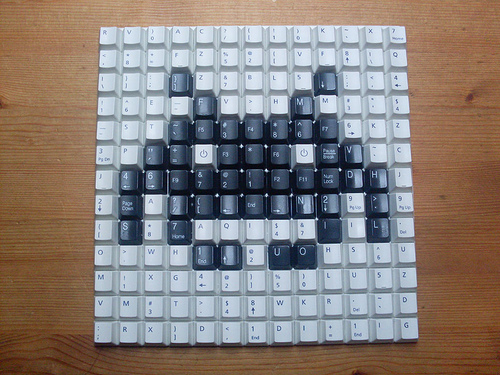
\includegraphics[scale=0.5]{images/spaceinvfun}
  \caption{Arte realizado por un fan.2002}
  \label{fig:arte}
\end{figure}

Poco después de ser liberado, \emph{Space Invaders} creció en popularidad. En 1980, se licencia para su uso en los Estados Unidos. Fue lanzado en las máquinas recreativas que funcionan con monedas como en la figura \ref{fig:ejemplo}, el Atari 2600, y la Nintendo Entertainment System. En su vida útil genero más de 500 millones de dólares en ingresos.\\
\begin{figure}
  \centering
    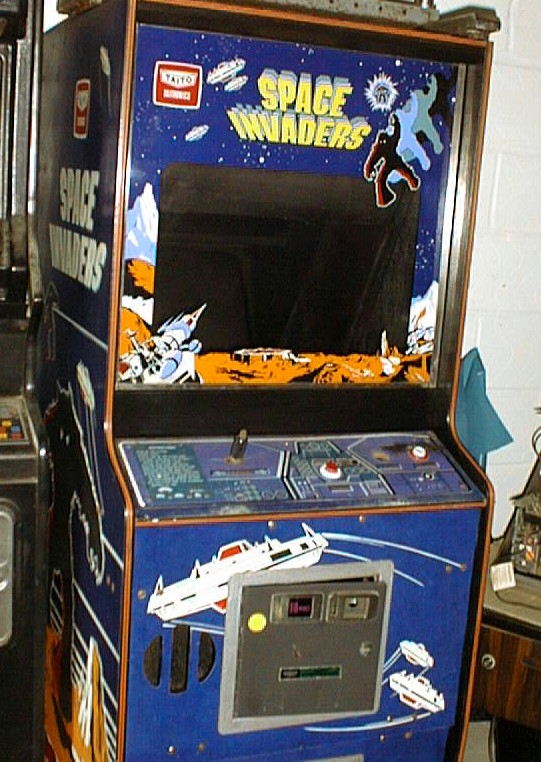
\includegraphics[scale=0.5]{images/machine}
  \caption{Maquina de Space Invaders, Taito 1978.}
  \label{fig:ejemplo}
\end{figure}

\subsection{Principio Basico}
Es un juego de acción en 2D donde un humano debe proteger la tierra de los extraterrestres. Hay 48 aliens en cada etapa que están uniformemente espaciadas en 6 columnas. Los aliens se mueven hacia izquierda y derecha a través de la pantalla en un patrón establecido, avanzando lentamente hacia la tierra. Es el trabajo del jugador humano disparar a todos los aliens antes de que lleguen a la tierra. Los aliens también disparan al azar, por lo que el jugador humano deben evitar esquivar ser fusilado por los aliens. Si el jugador humano es capaz de destruir los 48 aliens, entonces él o ella avanza a la siguiente etapa en la que tienen un nuevo conjunto de 48 aliens para destruir. Otro aspecto del juego es el conjunto de escudos prestados al jugador. En el juego hay 3 escudos que el jugador humano puede utilizar, para  esconderse detrás para evitar recibir un disparo por los extraterrestres. A medida que estos escudos reciben daño, disparos pueden penetrar a través de ellos.\\

Space Invaders se ha actualizado y puesto en libertad en muchas plataformas diferentes, pero todos han sido en forma de dos dimensiones estándar. Hasta el momento Taito nunca ha lanzado una versión en 3D del juego. Sin embargo, en 1999, Space Invaders fue re-lanzado para el Nintendo 64. Aunque los fondos y los personajes fueron diseñados en 3D, el juego sigue siendo un shooter en 2D.

\subsection{Iconos}
En internet existe una gran cantidad de recursos en linea que proveen sonidos, imagenes e iconos, en nuestro caso nosotros solo hemos utilizados dos sonidos obtenidos de aqui\footnote{http://www.classicgaming.cc/classics/spaceinvaders/icons.php} también de \footnote{http://www.softicons.com/game-icons/classic-games-icons-by-thvg/space-invaders-5-icon, SoftIcons} por supuesto se realizan las modificaciones pertinentes para obtener color y transparencias como se puede ver en la figura \ref{fig:iconos}.

\begin{figure}
  \centering
    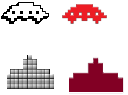
\includegraphics[scale=0.5]{images/iconos}
  \caption{Iconos Utilizados.}
  \label{fig:iconos}
\end{figure}

\section{Requisitos para Correr}

Para correr este juego se debe correr con la opción \textbf{Determine Language from Source}, para que el archivo del juego sea el que seleccione cual sera el lenguaje, para nuestro caso es \textbf{\#lang racket}  ademas de ello solo por seguridad puedes incrementar el limite de memoria de 128MB a 256MB llendo al menu de DrRacket como lo muestra la figura \ref{fig:ml} ,

\begin{figure}
  \centering
    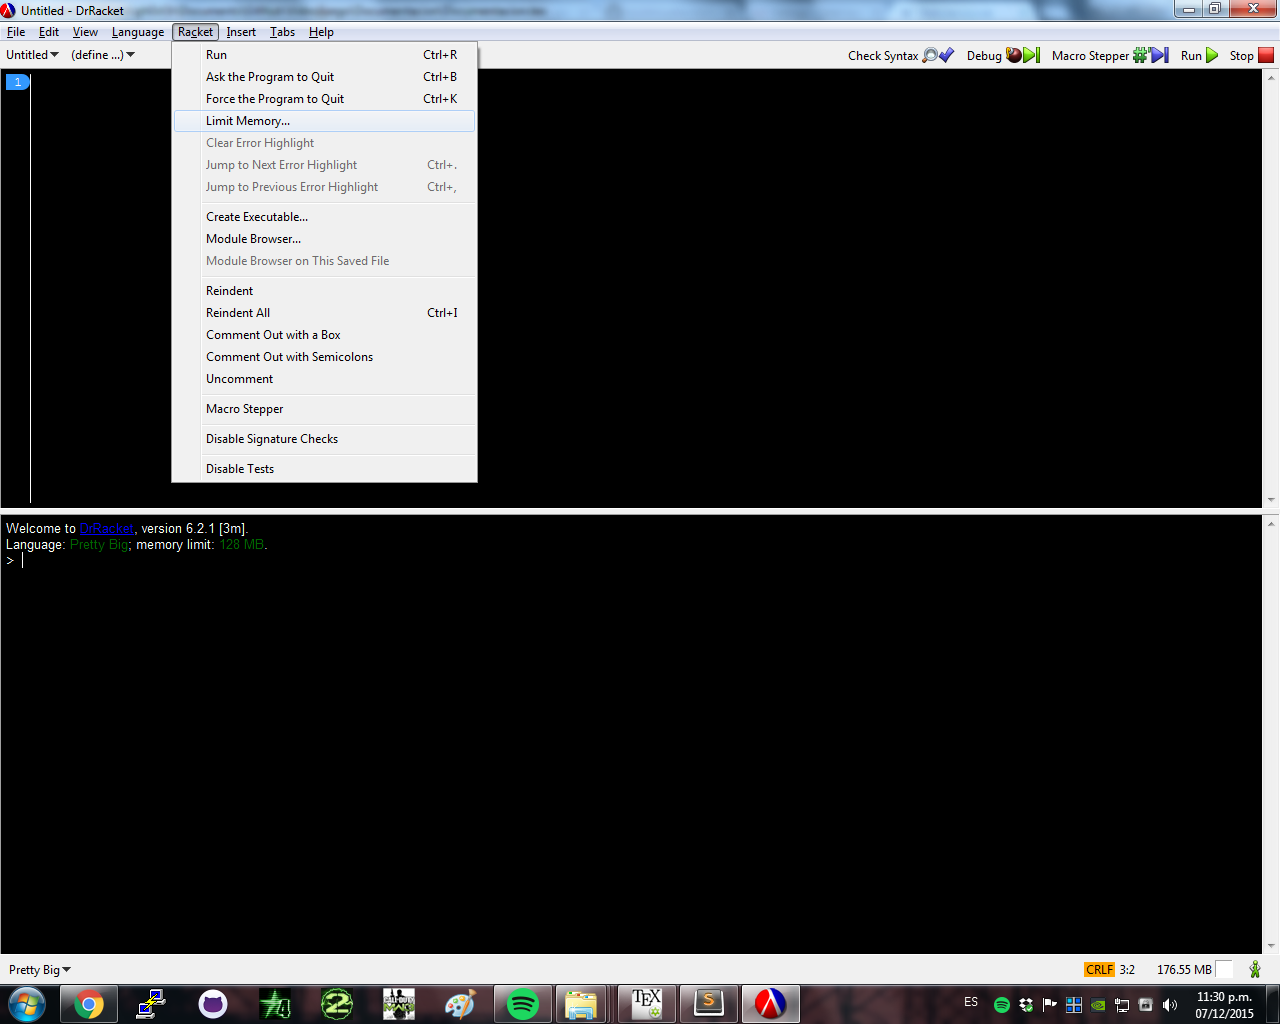
\includegraphics[scale=0.35]{images/limmemoria}
  \caption{Incrementar Cantidad de Memoria en \textbf{\textit{Drracket}}.}
  \label{fig:ml}
\end{figure}

Es estrictamente necesario que las siguientes lineas se ejecuten:
\begin{lstlisting}
\#lang racket
(require 2htdp/image)  
(require 2htdp/universe)
(require math)
\end{lstlisting}

El juego se encuentra \emph{probado} bajo la version 6.2.1 de \textbf{DrRacket} para correr en plataformas Microsoft Windows versiones \textit{ 7,8,8.1,10 Profesional},además  Distribuciones Gnu\/Linux \textbf{\textit{Debian}} y Derivados.
En caso de tener problemas consulte a los desarrolladores.
\begin{figure}
  \centering
    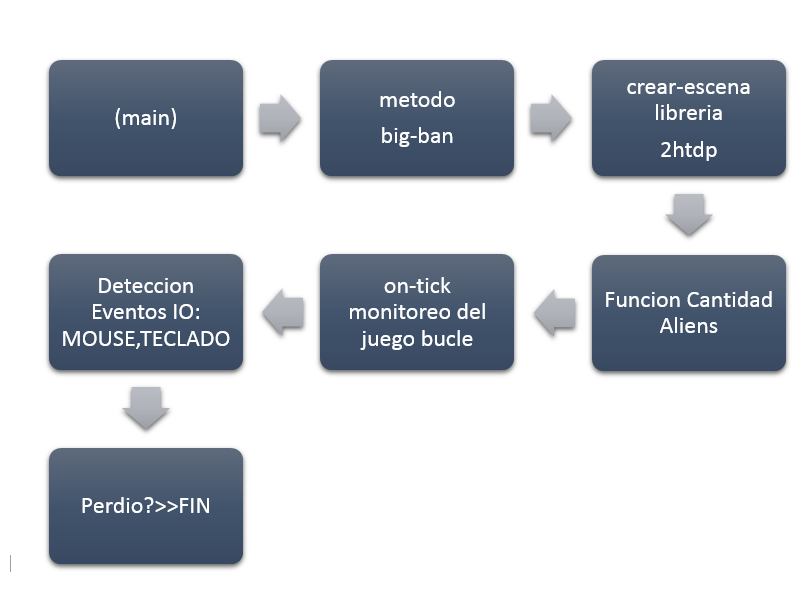
\includegraphics[scale=0.6]{images/smart}
  \caption{Llamado de Funciones, Ciclo infinito.}
  \label{fig:smart}
\end{figure}

\newpage
\section{Detalles Tecnicos de  DrRacket}
\label{sec:detecnicos}

Para el diseño de este juego y con el fin de poner en practica el concepto de \textit{divide and conquer}, se crearon múltiples funciones, de las cuales se mencionara las mas importantes, además un resumen del ciclo de llamado del juego se puede observar en el siguiente smart art presentado en la figura \ref{fig:smart}, en el cual solamente se ejecuta la primera vez la creación de escenas, utilizando 2htdp.
siguientes funciones:
\begin{description}
    \item[Comunicador m:] Se encarga de mostrar por pantalla la nave, y enviar los datos a otra función denominada \textit{mostrar-balas}
    \item[ver-aliens b:] Se encarga de mostrar los aliens por pantalla, con movimientos.
    \item[monitoreo :]Se encarga de cambiar los valores, también se utiliza para actualizar la posición de objetos, y crear objetos de manera temporizada. 
    \item[Cambia Posición Aliens:]Actualiza la posición de los aliens dentro de la ventana designada.	
    \item[Mouse] Maneja la posición de la nave utilizando el mouse, las posiciones de esta solo son en 1d 
        en el eje X, descarta las posición del mouse en Y,Z.
    \item[dificultad:]Cambia los parámetros del juego,que implica:
      \begin{itemize}
      \item Incrementar la velocidad de desplazamiento de la nave.
      \item Incrementa en uno el nivel del juego.
      \item Incrementa la intensidad de ataque de los aliens en juego.
      \item Incrementa la velocidad de movimiento de izquierda a derecha.
      \item Incrementa la velocidad de la bala.
      \item cambia de color de los aliens.
      \item coloca random de nivel para los aliens.
     \end{itemize}
\end{description}

\subsection{Creación de Ventanas}
Para la creacion de ventanas existian dos posibilidades que eran:
\begin{lstlisting}
\#lang racket
(require 2htdp/image) 
(require 2htdp/universe)
o
(require (lib graphics.ss  graphics) )
\end{lstlisting}
Nosotros realizamos las pruebas correspondientes con la librería \textit{graphics} pero al realizar las pruebas veíamos que existían muchos problemas, pues aquí la la clave es estar haciendo un juego entre ventanas, creamos una ventana, se pone el fondo necesario, y creo otra ventana encima de esa para hacer lo que se necesite, pero no es optimo y no saldría muy bien dado que para nuestra idea, necesitamos poner varias capas o ventanas a interactuar entre ellas. Se opto por la solución recomendada en la documentación de DrRaket que era utilizar dos paquetes de \textbf{2htdp \footnote{Documentación de Image.rkt, http://docs.racket-lang.org/teachpack/2htdpimage.html?q=2htdp}, \footnote{Documentación de universe.rkt, http://docs.racket-lang.org/teachpack/2htdpuniverse.html?q=2htdp}}. La gran ventaja aquí es que tu no te preocupas por el manejo de ventanas, sale muy bien por que tu creas la escena con la figura de fondo y encima de esa escena montas las demás funciones, figuras que necesitas poner a interactuar.
\subsection{Funcion Principal}
Resulta que para poder llamar las funciones que se encuentran descritas a continuación se debe hacer uso de un metodo definido en las librerias de universe, estamos hablando del metodo \textbf{\emph{big-bang}} que permite el llamado y actualización constante de varias funciones, la función principal se llama una sola vez, pero los llamados a las subfunciones se hacen constantemente gracias a la estructura que posee universe para realizar esto. a continuación se muestra el codigo resumido:
\begin{lstlisting}
;controla el mundo, el la encargada de enviar y recibir actualizaciones de 
;todas las funciones del juego
(define (main) 
(big-bang 
  (make-mundo 
   (/ ancho 2) 
   empty 
   enemigos
  )
 [on-tick monitoreo]
 [to-draw comunicador]
 [on-mouse mouse]
 [on-key teclado]
 [stop-when perdi? dar-final]
))

;inicio el juego
(main)
\end{lstlisting}
notece que del código anterior se definió una función main contenedora de las funciones mas destacadas de nuestro código, la primera vez que se llama a big-bang esta se encarga de crear el mundo que es una estructura, pero solamente se crea el entorno una sola vez, las siguiente funciones estan constantemente corriendo dentro de un loop, la funcion monitoreo hace un refresh del entorno y movimientos, presentados por el mouse y el teclado pues es sabido que toca mirar si se presiono o no el teclado y mouse. \textbf{\emph{[on-mouse mouse],  [on-key teclado]}}.
Finalmente la función  \textbf{\emph{[stop-when perdi? dar-final]}} se encarga de verificar si el usuario perdio, si esto es verdadero se llama la funcion dar-final que muestra en pantalla la imagen de game over.

Algunas notas importantes son :
\begin{lstlisting}
;El mundo se utiliza para que barias funciones interactuen simultaneamente 
;y se puedan embiar parametros de una forma facil, la funcion principal 
;(big-bang) embiala actualizaciones contantemente a cientas funciones,
;la estructula para usar es: 

;(define-struct identificador [rama1 rama2 ....])

;(big-bang identificador
;[aqui-caracteristica-a-emplear mi-funcion]
;[aqui-caracteristica-a-emplear mi-funcion2]
;big-bang envia todos los datos a las funciones secuencialmente

;para extraer los valores del mundo que definimos ariva hacemos 
;el llamado de cualquiera de las siguentes funciones
 ; (mundo-jugador a)
 ; (mundo-disparo a)
 ; (mundo-enemigos a)   
\end{lstlisting}
\subsection{Estructura Mundo}
Se utilizo una estructura de datos que permite una mejor manipulación de los datos, nosotros por podriamos tener una estructura que se llame \emph{\textbf{persona}} y tener diferente informacion de esta por ejemplo la cedula, telefono, año de nacimiento, asi que es posible que cada vez que nosotros accedamos a la estructura persona para agregar varias personas. Nosotros utilizamos lo mismo nosotros definimos una estructura denominada mundo asi :
\begin{lstlisting}
(define-struct mundo [jugador disparo enemigos])
\end{lstlisting}
Sabemos que son las cosas mas importantes y mas representativas dentro del juego.

\subsection{Constantes}
Durante el desarrollo de todo el código en DrRacket y a lo largo de el fue necesario utiliza variables constantes, que representan datos que no cambiaran durante el ciclo de ejecución de este, el siguiente fragmento de codigo muestra las constantes utilizadas:
\begin{lstlisting}
;Constantes  Detalles Tecnicos
(define ancho 780)    ;Define el ancho de la escena 
(define alto 500)
(define veloz-nave 25) ;Velocidad inicial de desplazamiento de la nave.
(define veloz-bala 15) ;Velocidad inicial de las balas disparadas por la nave.
(define veloz-aliens 5);Velocidad de los aliens
(define intencidad 1)  ;Cuando los aliens atacan, ellos tienen una intensidad de ataque.
;1 es lo mas basico en la intensidad de ataque.
(define proyectil (rectangle 5 10 "solid" "red"));Dibujamos el rentagulo de ancho 5,alto 10 relleno de rojo.
(define rango-acierto 20) ; Esta es la distancia inicial que existe entre un alien y la bala, si la distancia es cercana a 20 el alien se destruye.
(define en-fondo .) ;fondo       ;Fondo de Estrellas.
(define game-over-im .)          ;Fondo de game-over imagen
(define nave1 .)                 ;Imagen  nave1
(define nave2 .)     			 ;Imagen  nave2
(define aliens1 .)    		;Imagen  aliens1 color blanco
(define aliens2 .)     		;Imagen  aliens2 color rojo

;posibilidad de ataque enemigo
(define int (truncate (/ ancho  intencidad))) 

;nivel del juego inicial y puntuacion
(define nivel 1)
(define puntuacion 0)

\end{lstlisting}
\subsubsection{Constantes:Sonidos}

También se define algunos sonidos que serán constantes como:
\begin{lstlisting}
(define (disparo) (play-sound "Sounds/shoot.wav" #t))         ;Esto va a reproducir  el nombre de archivo completo, el sonido es corto.
(define (explosion) (play-sound "Sounds/explosion.wav" #t))   ;
(define (invaderlejos) (play-sound "Sounds/invlejos.wav" #t)) ;
(define (menu) (play-sound "Sounds/menu.wav" #t))             ;recortado a 10 segundos.
\end{lstlisting}
Para reproducir utlizamos la funcion \textbf{\emph{play-sound}} que se encuentra en \textbf{racket/gui/base} que basta con decirle la ubicación del archivo .wav,.mp3 y un true(\textbf{\#t}) o false(\textbf{\#f}) para reproducir. Aquí también encontramos que existe un problema, pues si el sonido es muy largo la reproducción queda sonando adueñándose del driver de sonido en cualquiera de los sistemas operativos probados probados.
\subsection{Dificultad}
Como se mencionaba en el parrafo de \ref{sec:detecnicos} esta funcion basicamente cambia todos los parametros de dificultad, el siguiente codigo muestra como se cambia:
\begin{lstlisting}
(define (dificultad a)
 (begin 
  (set! veloz-nave (+ veloz-nave 4))
  (set! nivel (+ nivel 1))
  (set! intencidad (+ intencidad 1))
  (set! veloz-aliens (+ veloz-aliens 1))
  (set! veloz-bala (+ veloz-bala 1))
  (if 		            ;Si el nivel es 4 cambia el color de los aliens 
   (= nivel 4)              ;Comparador.
   (set! aliens1 aliens2)   ;setea de figura aliens1 a aliens2
   ""
  )     
  (* 20 (+ 1 (random nivel)))  ;random para nivel de ataques...
  )
 ) 
\end{lstlisting}

\subsection{Crear Enemigos: Aliens}
Esta función se encarga de crear una lista que contendrá varias listas así es posible establecer una cantidad mínima de  aliens(\textit{enemigos}). 
\begin{lstlisting}
(define enemigos 
 (list 
  (list (random ancho) 20 #t) 
  (list (random ancho) 40 #f) 
  (list (random ancho) 60 #t)
  (list (random ancho) 80 #f)
 )
)
\end{lstlisting}
Una vez creados los enemigos debemos enviar los enemigos al procedimiento necesario, y cuando sea estrictamente necesario agregaremos mas aliens, el siguiente código 
\begin{lstlisting}
;envia la lista de enemigos y agrega un enemigo
(define (dame-enemigos a) 
 (begin
  (set! enemigos        ;Setea la posicion de los aliens
   (cons 		;Este par conecta los aliens con los previos
    (list (random ancho) (dificultad ";)") #t)
    enemigos
   )               
  )
  enemigos  
 )
)
\end{lstlisting}
\subsubsection{Movimiento de Izquierda a Derecha de los Aliens}
Para generar un movimiento interactivo de los aliens, se debe realizar un recorrido por toda la ventana de la escena,  e ir desplazando las listas sabemos que para acceder las listas se puede hacer uso de varias conbinaciones como \textbf{car, cdr}, o mezcladas. y los pares juntos, también algunas veces es necesario que los aliens ataquen es depende directamente del nivel de intensidad y dificultad:

A continuación se pone el código utilizado para el movimientos de los aliens, izquiera - derecha abajo.

\begin{lstlisting}
;cambia la posision de los aliens:
;la funcion busca que los aliens bajen en un
;momento aleatorio
;(mover-aliens mundo-enemigo)

(define (mover-aliens a)
 (cond
  [(empty? a) empty]
  ;hace que los alien bajen
  [(number? (car (cddar a))) 
   (cons
    (list 
     (caar a)
     (+ (cadar a) veloz-aliens)
     (car (cddar a))
    )
    (mover-aliens (cdr a))
   )
  ]
  ;mueve a la derecha
  [(car (cddar a)) 
   (cons  
    (list     
     (+ (caar a) veloz-aliens )
     (+ (cadar a) 0)
     (if (> ancho (caar a)) 
      (if (= 1 (random int))
       (+ 20 (random (- ancho 20)))
       #t
      )       
       #f
      )      
     )                      
    (mover-aliens (cdr a))
   )
  ]
  ;mueve a la izquierda
  [(not (car (cddar a))) 
   (cons  
    (list 
     (- (caar a) veloz-aliens)
     (+ (cadar a) 0)
     (if (> (caar a) 20)
      (if (= 1 (random int))
       (+ 20 (random (- ancho 20)))
       #f
      )
      #t
     )
    )                  
    (mover-aliens (cdr a))
   )
  ]
 )  
)
\end{lstlisting}
\subsubsection{Eliminar Aliens Muertos}
Para eliminar los aliens que han sido eliminados por una bala se debe tomar la lista de aliens  eliminar un elemento de ahí, \textbf{\emph{pero como saber cual es el elemento que ha sido golpeado por la bala ?}}, lo que se puede hacer es encontrar la distancia que existe entre dos puntos, el primer punto \textbf{A(x1,y1)} sera la bala, y el segundo sera la posición de los aliens que estan determinadas en la lista \textbf{B(x2,y2)}

\begin{lstlisting}
;remover los aliens muertos
(define (remover-aliens enemigo bala)
 (cond
  [(empty? enemigo) empty]
  [(cons? enemigo) 
   (cond
    [(cerca-aliens? (car enemigo) bala) (remover-aliens (cdr enemigo) bala)]
    [else (cons (car enemigo) (remover-aliens (cdr enemigo) bala))]
   )
  ]
 )
)
;---------------
;dice si la bala impacto o no contra el aliens
(define (cerca? e d)
 (cond
    [(<= (distancia e d) rango-acierto) ;rango acierto es una constante
     (begin
       (set! puntuacion (+ 10 puntuacion)) (explosion) #t
       )
     ]
    [else #f])  
)

\end{lstlisting}

\subsection{Funciones de Movimiento}
Hay dos funciones principales de movimiento, ellas son las encargadas de leer si se presiono o no las teclas de \textbf{izquierda,derecha o espacio para disparar}, la además el usuario también tiene la posibilidad de útilizar el mouse y el click izquierdo para disparar, en esta funcion se descartan los movimientos del mouse en Y, pues la nave solo es posible moverla en x entre los limites dados en las constantes.
\begin{lstlisting}

;manejo con mouse
;datos-mundo   pos-x   pos-y tipo-de-evento -> (en la ventana)
(define (mouse m x y estado) 
 (cond
  ;lee posision horizontal del mouse
  [(string=? estado "move") 
   (make-mundo
    x 
    (mundo-disparo m) 
    (mundo-enemigos m)
   )
  ]
  ;lee clic
  [(string=? estado "button-down") 
   (make-mundo 
    (mundo-jugador m)                                             
    (agregar-bala x (mundo-disparo m))                                              
    (mundo-enemigos m))]
  [else m]
 )
)
;---------------------
;manejo con el teclado
(define (teclado m tecla) 
 (cond
   ;lee flecha izquierda  
   [(and (equal? tecla "left") (> (mundo-jugador m) 20) )
   (make-mundo    
    (- (mundo-jugador m) veloz-nave) 
    (mundo-disparo m) 
    (mundo-enemigos m)
   )
  ]
  ;lee fecha derecha  
  [(and (equal? tecla "right")(< (mundo-jugador m) (- ancho 20)))
   (make-mundo    
    (+ (mundo-jugador m) veloz-nave) 
    (mundo-disparo m) 
    (mundo-enemigos m)
   )
  ]
  ;leer tecla espacion (para disparar)
  [(equal? tecla " ") 
    (make-mundo 
     (mundo-jugador m)                                             
     (agregar-bala (mundo-jugador m) (mundo-disparo m))                                              
     (mundo-enemigos m)
    )
  ]
  [else m]
 )    
)
\end{lstlisting}

Hay que notar que las funciones siempre se estan enviando un parametro de actualizacion entre ellas misma, esta es utilizada por monitoreo(\ref{fig:smart}).
\subsection{Funciones de Disparo}
Para las balas se utilizo un par que permite concatenar la bala en la nueva posicion, como se muestra a continuacion.

\begin{lstlisting}
;agrega una bala en la lista de balas. 
(define (agregar-bala x viejas-balas)
 (begin
   (disparo)
   (cons 
  (list x (- alto 40)) 
  viejas-balas
 ))  
)
\end{lstlisting}

\clearpage
\newpage
%Toolset.
\section{Links de Paginas de Interés \label{Herramientas}}
\begin{itemize}
\item \href{https://github.com/stuhlmueller/scheme-listings}{Resaltar Codigo Scheme en \LaTeX}
\item \href{http://docs.racket-lang.org/teachpack/2htdpimage.html?q=2htdp}{image.rkt, Paquete para el manejo y dibujo de imagenes}
\item \href{http://docs.racket-lang.org/guide/module-basics.html}{Manejo de Librerias Propias, Estructura.}
\item \href{http://https://github.com/darrencruse/pong-world-racket}{Ejemplo de Ping Pong World.}
\item \href{http://austinmaddocks.weebly.com/drracket.html}{Juegos de Ejemplos, Grupo de Hackers Austin.}
\item \href{http://docs.racket-lang.org/games/}{Juegos Oficiales de DrRacket}
\item \href{http://docs.racket-lang.org/teachpack/2htdpPlanet_Cute_Images.html}{Imagenes Prediseñadas en DrRacket.}
\item \href{https://github.com/buntine/Simply-Scheme-Exercises}{Ejercicios de DrRacket Resueltos.}
\item \href{https://github.com/}{Github el Facebook de los hackers.}
\item \href{https://try.github.io/levels/1/challenges/1}{Guia del Controlador de Versiones Git.}
\item \href{https://github.com/davexunit/gnumaku}{Motor de Balas en 3D usando DrRacket.}
¡Gracias!
\end{itemize}

\clearpage
\section{Adjuntos}
Adjuntamos las imagenes y figuras (\ref{fig:inicio}),(\ref{fig:incrementonivel}), (\ref{fig:finalperdio}) de la version final, ademas de ello el código puede se encontrado en : \textbf{\href{github.com/heticor915/VideoJuego}{Space Invaders Version Final.}}
\begin{figure}
  \centering
    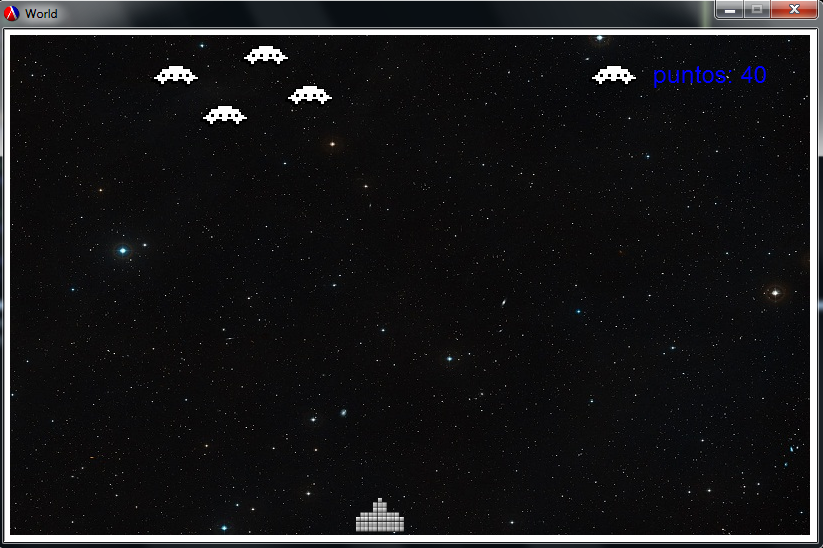
\includegraphics[scale=0.4]{images/inicio}
  \caption{Version Juego Final, Usuario empieza en nivel 1 \textbf{\textit{Drracket}}.}
  \label{fig:inicio}
\end{figure}

\begin{figure}
  \centering
    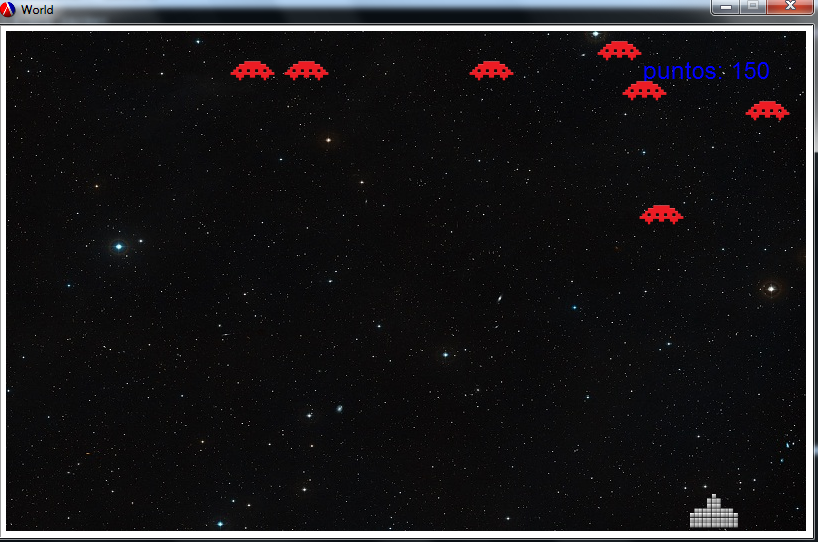
\includegraphics[scale=0.4]{images/nivelinc}
  \caption{Version Juego Final, Usuario avanza a mas nivel, nivel 5 \textbf{\textit{Drracket}}.}
  \label{fig:incrementonivel}
\end{figure}

\begin{figure}
  \centering
    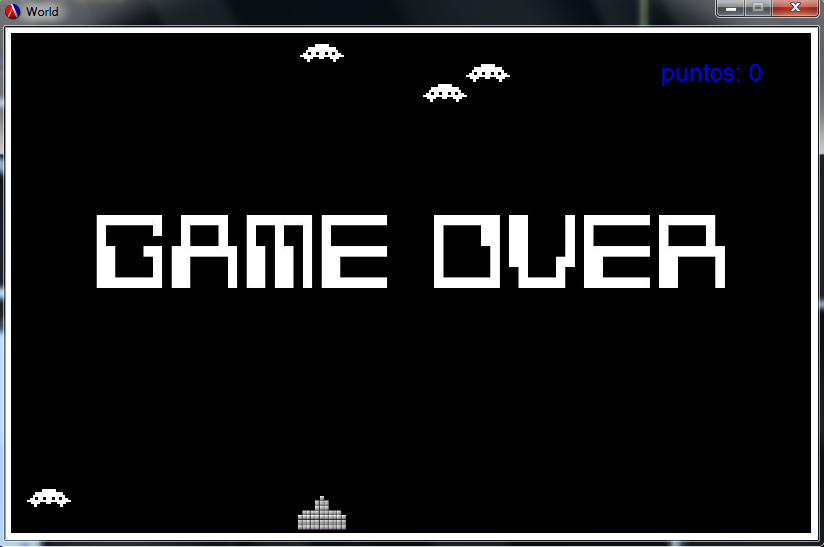
\includegraphics[scale=0.7]{images/fin}
  \caption{El Usuario Perdio \textbf{\textit{Drracket}}.}
  \label{fig:finalperdio}
\end{figure}

\clearpage
\newpage
\section{Agradecimientos}
Los autores \textbf{\emph{Brian Ruiz Idarraga, Héctor F. Jiménez Saldarriaga}}desean agradecer a la Universidad Tecnológica de Pereira, al programa de Ingeniería de Sistemas y Computación y al profesor \textbf{Francisco Medina} por haber asesorado en las consultas y dudas presentadas durante el desarrollo de este juego. También agradecer a todos aquellos que ofrecieron sus opiniones y consejos durante el desarrollo de este.

Esperamos que el juego halla gustado si tienes alguna duda escríbenos a nuestros mails.
\end{document}



